\documentclass[10pt]{iopart}
\include{setup}

\begin{document}
\ioptwocol[{
\title[A lagrangian mechanics oriented approach to neural networks]{A lagrangian mechanics oriented approach to neural networks}
\author{A S Roberts}
\address{Department of Physics, University of Bath, Claverton Down, Bath BA2 7AY, UK}
\begin{abstract}
\lipsum[1]
\end{abstract}
}]
% Four main areas of focus:
% 1. Neural Networks in Physics
%		- Neural Networks 101 - DONE
%		- Neural Networks in Physics
%			- PNN
%			- NN for Physics
%		- Things we can work with
%			- Loss Function
%			- Model
%			- Data
% 2. Slimplectic Integrator
% 		- Introduce Integrators
%			- Specialise to Slimplectic
%			- Explain Slimplectic
%		- Talk about Optimisation	
% 		- GPU applications	
% 3. Loss Functions
% 4. LMNN
\section{Introduction}
\subsection{Neural Networks in Physics}
Machine learning has become the latest addition to the modern physicists toolkit with a broad range of applications from deep learning for imaging in medical physics \cite{MedPhysDL} to large scale data analysis in astrophysics \cite{astroML}. Machine learning and often neural networks are allowing physicists to tackle problems which were previously intractable due to the size and scale of the computational required. To understand how this tool can be used one must first understand how the tool works.

Neural networks are the most common form of machine learning and work by finding a generalised non-linear function (the neural network) between the input and output spaces. The input space is the space of data in which patterns aim to be discovered. For medical imaging this might be pixel values for a certain size image or in astrophysics it may be a range of luminosity values attributed to certain wavelengths of light. The output space is similar, a space of possible outputs such as possible classifications of an astrophysical object with respective confidence levels.

 One of the main draws of neural networks is the ability to apply the function to any object in the input space, even if previously unseen. The neural network can be seen as a connected graph where each node and connection has a weighting (weights and biases respectively). To obtain a function that can accurately predict an outcome for any element of the input space the neural network has to be trained. This training involves taking a known subset of the input and output spaces called the training data set along with a loss function $f_{\mathrm{loss}}$. The loss function compares the neural networks calculated outputs with the known (true) outputs in the training data. Starting with a randomly initialised neural network (randomised weights and biases) the following process can be repeated to slowly optimise the network:
 
 \begin{enumerate}
 	\item Pass an element of the training data through the neural network
 	\item Calculate losses for the output
 	\item Take the gradient of the loss function with respect to the weights and biases in the neural network
 	\item Update the weights and biases according to $-\nabla f_{\mathrm{loss}}$ to minimise the loss of the function
 \end{enumerate}
 
By repeating this process local minima of the loss function can be found thereby optimising the neural network. 
Ideally, a global minima would be found but this is not guaranteed by the method outlined above. Optimisation algorithms such as Adaptive Moment Estimation (ADAM) optimiser \cite{ADAM} can be implemented in order to increase these chances by varying the size of the updates made when taking the gradient of the loss function.

With the ability to identify possibly unseen patterns in data, neural networks are an ideal tool for physicists. One area of neural network development related to this is that of physics informed neural networks (PINN's). These are neural networks that have been given a priori knowledge such as basic physical laws. This knowledge can be encoded into the model in a multitude of ways. Physics informed layers of the neural network are one such encoding such as layers that enforce conservation laws for fluid dynamics. Another encoding is via loss function formulation where the loss function incorporates terms derived from the governing physics equations. These terms will act to penalise the model for deviation from known physical laws. 

\subsection{Loss Functions}
Loss functions play a crucial role in PINNs often acting as a conduit for incorporating known physical laws. PINN loss functions usually have two purposes:
\begin{itemize}
	\item Data Fitting: This ensures that the network accurately predicts values, much like in more general neural networks.
	\item Physics Information: An encoding of physical laws such as ensuring specific PDE's are satisfied by penalising deviation from governing equations. 
\end{itemize}

One issue that loss functions face is the requirement of being differentiable with respect to the weights and biases of a network. This often leads to simple regression functions such as mean squared error being selected in order to guarantee this property. A regression function may be paired with a simple physics informed term such as a penalisation of deviation from conservation terms. For example, conservation of mass within fluid dynamics for an ideal fluid can be expressed as 
\begin{equation}
\label{FluidConservation}
	\nabla \cdot\dot q = 0
\end{equation}
 
so a penalisation term in the loss function could be written as Conservation term $=\Lambda|\nabla \cdot \dot q|^2$ thus penalising deviation from equation \ref{FluidConservation}.

Another more applied issue that loss functions face is coding efficiency restraints. As on of the most called functions within the neural network training process a loss function is constrained to mathematically quick calculations and there often cannot afford to implement longer more involved calculations. 

\subsection{Google JAX}
Google JAX \cite{Jax} is a python machine learning framework developed by Google that collates the properties of Autograd \cite{Autograd} and XLA (Accelerated Linear Algebra) \cite{XLA} which include just in time (JIT) compilation). Autograd allows for automatic differentiation of both \texttt{python} and \texttt{NumPy} functions, a beneficial property when performing gradient descent during training of neural networks. JIT compilation allows functionally written pieces of python code to be converted from interpreted to compiled code. By JIT compiling code is converted into mathematically more efficient ''black-box" functions which map inputs to outputs in less time. This is especially beneficial for code that is frequently called as it need only be JIT compiled once before the ''black-box" version is  used thereafter.


\subsection{Lagrangian Mechanics}
Here we provide a brief overview of Lagrangian Mechanics, a formalism of classical mechanics prioritising the energy of a system as its initial reference point. 

Lagrange's formalism considers a set of generalised coordinates $\{q_1,q_2,\ldots,q_n,\dot{q}_1,\dot{q}_2,\ldots,\dot{q_n},t\}$(hereon denoted as the vectors $\bold{q}$ and $\bold{\dot{q}}$) which are used to express the kinetic, $T$, and potential, $V$, energies of the system. The Lagrangian 
\begin{equation}
	\mathcal{L}(\bold{q},\bold{\dot{q}},t) = T(\bold{q},\bold{\dot{q}},t) - V(\bold{q},\bold{\dot{q}},t)
\end{equation}

\noindent is defined as the difference between the two energies of the system. The Lagrangian provides the final object of interest the action, $S$, defined as

\begin{equation}
		S = \int_{t_1}^{t_2} \mathcal{L}(\mathbf{q},\mathbf{\dot{q}},t) dt
\end{equation}

\noindent a functional of which stationary points are of interest. Hamilton's principle \cite{Goldstein} that these stationary points are where the Lagrangian models physical reality i.e. $\delta S = 0$. 

From here the equations of motions (EoMs) can be obtained by applying the Euler-Lagrange equation which is equivalent to minimising the action (and thus finding its stationary points)

\begin{equation}
\label{Eul-Lag}
	\frac{\partial\mathcal{L}}{\partial q_i} - \frac{d}{dt}\left(\frac{\partial \mathcal{L}}{\partial \dot{q_i}}\right) = 0
\end{equation}

\noindent where we obtain $n$ differential equations for the $n$ generalised coordinates. Equation \ref{Eul-Lag} then provides a generalised form for the EoMs of a conservative system. 

Much like generalised coordinates and velocity, generalised momenta is introduced here as 

\begin{equation}
\label{GeneralisedMomenta}
	p_i = \frac{\partial \mathcal{L}}{\partial \dot q}
\end{equation}

and is the fundamental basis for all forms of momentum, both linear and angular.

\subsubsection{Example: Simple Harmonic Oscillator \\}

A motivating example may be that of the 1-dimensional simple harmonic oscillator given by the differential equation

\begin{equation}
	\ddot x = x
\end{equation}
with position $x$, mass $m$ and spring constant $k$. The kinetic energy of this system is then given by
\begin{equation}
	T = \frac{1}{2}m\dot x^2
\end{equation}
and the potential energy by 
\begin{equation}
	V = \frac{1}{2}kx^2
\end{equation}

\noindent This gives the lagrangian
\begin{equation}
	\mathcal{L} = \frac{1}{2}m\ddot x^2 - \frac{1}{2}kx^2
\end{equation}

\noindent which when inputted into equation \ref{Eul-Lag} once again provides our known equation of motion
\begin{equation}
	\ddot x = \frac{k}{m}x
\end{equation}\

Conservation laws can also be identified through the use of lagrangian mechanics via Noether's Theorem \cite{Goldstein}. It states that every differentiable symmetry of the action for a conservative system has a corresponding conservation law. The conserved values are often known as Noether currents when considered as functions of time. 

\subsubsection{Nonconservative Lagrangians \\}
Galley, Tsang and Stein \cite{GalleyEtAl} propose a generalisation of Noether's Theorem to allow for non-conservative systems. This works by generalising to the nonconservative lagrangian, $\Lambda$, of the form 

\begin{equation}
\label{non-con-lagran}
	\Lambda = \mathcal{L}(\bold{q_1,\dot q_1},t) - \mathcal{L}(\bold{q_2,\dot q_2},t) + K(\bold{q_1,\dot q_1,q_2,\dot q_2},t)
\end{equation}

where $\mathcal{L}$ is the lagrangian as defined previously and $K$ is an additional coupling term physically similar to a non-conservative potential. The generalised coordinates are doubled, as explained by Galley \cite{Galley}, from $\bold{q,\dot q}$ to $\bold{q_1,\dot q_1, q_2, \dot q_2}$. This allows for the conversion of Hamiltons principle from a boundary value problem (i.e. ``minimise the action passing through given initial and final values") to an initial value problem involving twice the degrees of freedom. These new generalised coordinates must satisfy $q_1(t) = q_2(t)$ and $\dot q_1(t) = \dot q_2(t)$ for $t \in \{t_i, t_f\}$. The cartoon in figure \ref{doubledCoords} depicts this doubling of coordinates to create a free end point.

Galley \cite{Galley} also shows that $K$ must be antisymmetric in swapping the indices and therefore must also vanish for $\bold q_1 =\bold q_2,\bold{\dot q_1} =\bold{\dot q_2}$.

\begin{figure}
	\label{doubledCoords}
	\centering
	\includegraphics[width=0.9\columnwidth]{Pingu.jpg}
	\caption{A cartoon depicting the doubling of coordinates posited by Galley \cite{Galley}. (a) shows a conservative system where initial and end points are fixed such that the solid path between them minimises the Action and dashed paths represent paths that do not minimise the Action. (b) shows a system with doubled coordinates. the point on the $t=t_f$ line is now free to vary but both the $q_{1,i}$ and $q_{2,i}$ points are fixed on the $t=t_i$ line. Here the $q_f$ point varies in order to globally minimise both paths. The physical limit occurs as $q_{2,i}\to q_{1,i}$ and, assuming the same system is modelled in both (a) and (b), rediscovers the path shown in (a).}
\end{figure}

For convenience a change of coordinates is often performed due to physical motivation. These are $q_- = (q_1 - q_2)/2$ and $q_+ = (q_1 + q_2)/2$  where the former can be considered a hypothetical displacement that vanishes in the physical limit $q_- \to 0$ and the latter the physically relevant component of the coordinates.
Note here that equation \ref{non-con-lagran} continues to satisfy the Euler Lagrange equation (equation \ref{Eul-Lag}) when evaluated in the physical limit (PL). This is formulated as

\begin{equation}
\label{NonConEulerLagrange}
	\frac{d}{dt} \left[\frac{\partial \Lambda}{\partial \dot{q_-}}\right]_{PL} - \left[\frac{\partial\Lambda}{\partial q_-}\right]_{PL} = 0
\end{equation}

\subsubsection{Hamiltonian Mechanics \\}
Another formulation of classical mechanics similar to lagrangian mechanics is that of Hamiltonian mechanics. As the name suggests the object of interest here is the classical Hamiltonian $H$ defined as 
\begin{equation}
\label{Hamiltonian}
	H = T + V
\end{equation}

Hamiltonian mechanics exchanges the use of generalised velocities $(\dot q)$ in favour of generalised momenta $p$. This is sometimes, but not always, equivalent to momenta in classical mechanics in the same way that $\dot\theta$ could be considered a velocity (time derivative of a coordinate $\theta$) but would not likely be ones initial idea for a velocity. This exchange does not affect the class of physical phenomena that can be described by Hamiltonian mechanics compared to Lagrangian mechanics; that is to say that these classes of phenomena are equivalent.

The Hamiltonian (equation \ref{Hamiltonian}) produces first order ordinary differential equations (ODEs) as the equations of motion

\begin{equation}
	\frac{dq_i}{dt} = \frac{\partial H}{\partial p_i}, \frac{dp_i}{dt} = -\frac{\partial H}{\partial q_i}
\end{equation}

This formulation is often useful for symplectic integrators \cite{SanzSerna} as discussed in section \ref{Symplectic}.

\section{Slimplectic Integrator}
\label{Symplectic}
Integrators are another tool within the modern physicists toolbox. Many physics problems have non-analytic solutions and this is where integrators make their appearance. Many integrators exist and are specialised for different applications. The Runge-Kutta method \cite{RungeKutta} is a well known and widely applied group of methods used for a balanced trade off between accuracy and efficiency. RK45 is perhaps paramount of these with an efficient method of finding solutions to problems with stronger than 4th order accuracy. One issue that Runge-Kutta faces however is that of compounding error. Whilst any one term has bounded error when using Runge-Kutta for integration, the total accumulation of error is not bounded causing issues for systems evolved over longer time periods. 

A remedy to this is another class of integrators called Symplectic integrators. These preserve (up to computational rounding) the differential 2-form called the symplectic form. Preservation of the symplectic form is analogous to preservation of certain physical constants. Due to this preservation the symplectic integrator is often used in integration of systems over long time scales. This is particularly common in orbital mechanics \cite{WISDOM, ReinTamayo} but also finds uses in statistical algorithms \cite{Neal_MCMC}.

One construction of symplectic integrators is via the means of variational integrators which are determined by the variation of a discretised action. This differs from traditional numerical integrators, such as Runge-Kutta, which discretises the equations of motion themselves. 


\begin{figure}
	\label{VariationalIntegrator}
	\centering
	\includegraphics[width=0.9\columnwidth]{Pingu.jpg}
	\caption{The difference between discretising a standard integrator and a variational integrator. In discretising a standard integrator the discretisation acts directly on the EoM's. However, a variational integrator discretises the action before determining the discretised EoM's.}
\end{figure}
\todo{fix figure}

Symplectic integrators are often used to solve Hamiltonian systems numerically. One common approach used for symplectic integrators is splitting methods such as the leapfrog and Verlet \cite{Verlet} methods. These work by splitting the Hamiltonian into smaller, more manageable parts and iteratively solving the system. By splitting the Hamiltonian like this the integrator can approximate solutions whilst preserving important geometric properties (such as the symplectic form, volume or energy) at a global level.

\subsection{The "Slimplectic" Integrator \\}
Tsang et al. \cite{Tsang_Slimplectic} have developed a variational integrator, the "Slimplectic" integrator, from the nonconservative action principle \cite{GalleyEtAl}. Starting with equation \ref{NonConEulerLagrange} the action integral $S = \int_{t_i}^{t_f}\Lambda(q_{\pm},\dot{q_{\pm}},t)dt$ is discretised using Galerkin-Gauss-Lobatto (GGL) quadrature \cite{GGL} as shown in figure \ref{GGLDiscretisation}. The GGL quadrature is chosen as it is an even order method and therefore symmetric under time reversal ($t\to-t$). The interval $t\in [t_n, t_{n+1}]$ has $r+2$ quadrature points given by

\begin{equation}
\label{timeDiscretisation}
	t_n^{(i)} \equiv t_n + (1+x_i)\frac{\Delta t}{2}
\end{equation}

where $\Delta t = (t_{n+1}-t_n)/2$, $x_0 \equiv -1, x_{r+1} \equiv 1$ and $x_i$ is the $i$th root of $dP_{r+1}/dx$, the derivative of the $(r+1)$th Legendre polynomial $P_{r+1}(x)$. 

\todo{Replace Image}
\begin{figure}
	\centering
	\label{GGLDiscretisation}
	\includegraphics[width = 0.9\columnwidth]{Pingu.jpg}
	\caption{The discretisation of time used within the GGL method. This is used to approximate the action to N timesteps between $t_i$ and $t_f$. Between $t_n$ and $t_{n+1}$ the quadrature discretises $r$ times as according to equation \ref{timeDiscretisation}.}
\end{figure}

To obtain approximations of values for $\dot{q}_{n,\pm}^{(i)}(t)$ at the quadrature points the derivative matrix \cite{Boyd}

\begin{equation}
	D_{ij} = 
	\begin{cases}
		-(r+1)(r+2)/(2\Delta t) &i=j=0 \\
		(r+1)(r+2)/(2\Delta t) &i=j=r+1 \\
		0 &i=j\notin\{0,r+1\} \\
		\frac{2P_{r+1}(x_i)}{P_{r+1}(x_j)(x_i-x_j)\Delta t} &i\neq j
	\end{cases}
\end{equation}
	
is used to give

\begin{equation}
	\dot{q}_{n,\pm}(t_n^{(i)}) \simeq \sum_{j=0}^{r+1} D_{ij}q_{n,\pm}^{(j)}
\end{equation}

where Tsang et al. \cite{Tsang_Slimplectic} provides more explanation as to the reasoning for this approximation.

 GGL quadrature allows any functional $\int F dt$ to be approximated over an interval of time by a discrete functional $F_d$ given by
 
\begin{equation}
\label{discretisedFunctional}
\begin{aligned}
F_d^n &\equiv F_d\left(q_{n, \pm},\left\{q_{n, \pm}^{(i)}\right\}_{i=1}^r, q_{n+1, \pm}, t_n\right) \\  &\equiv \sum_{i=0}^{r+1} w_i F\left(q_{n, \pm}^{(i)}, \dot{\phi}_{n, \pm}^{(i)}, t_n^{(i)}\right),
\end{aligned}
\end{equation}

where $w_i$ is a weighting given by 

\begin{equation}
	w_i \equiv \frac{\Delta t}{(r+1)(r+2)[P_{r+1}(x_i)]^2}.
\end{equation}

With a discretisation of $\dot{q}_{\pm}$ the action can be discretised by applying the methodology of equation \ref{discretisedFunctional} to equation \ref{non-con-lagran} defined as 


\begin{equation}
\mathcal{S}_d\left[t_0, t_{N+1}\right] \equiv \sum_{n=0}^N \Lambda_d\left(q_{n, \pm},\left\{q_{n, \pm}^{(i)}\right\}_{i=1}^r, q_{n+1, \pm}, t_n\right).
\end{equation}

This can then be applied to the the Euler Lagrange equation to obtain discretised equations of motion


\begin{subequations}
\label{positionEoM}
\begin{align}
		\left[\frac{\partial \Lambda_d^{n-1}}{\partial q_{n,-}} + \frac{\partial\Lambda_d^n}{\partial q_{n,-}}\right]_{PL} &= 0 \\
	\left[\frac{\partial\Lambda_d^n}{\partial q_{n,-}^{(i)}}\right]_{PL} &= 0.
\end{align}
\end{subequations}

Taking the definition of generalised momenta in equation \ref{GeneralisedMomenta}, discretised momenta can now be introduced by splitting equation \ref{positionEoM}a into 

\begin{subequations}
\label{slimplecticEqns}
\begin{align}
\pi_n &\equiv -\left[\frac{\partial\Lambda_d^n}{\partial q_{n,-}}\right]_{PL} \\
\pi_{n+1} &\equiv \left[\frac{\partial\Lambda_d^n}{\partial q_{n+1,-}}\right]_{PL} \\ 
0 &\equiv \left[\frac{\partial\Lambda_d^n}{\partial q_{n,-}^{(i)}}\right]_{PL}
\end{align}
\end{subequations}

which finally produces a set of discretised equations that can be computationally solved for. By taking initial conditions for $q_0, \pi_0$ the integrator can then forward integrate the system for N iterations whilst preserving (up to a constant error bound) 

Tsang et al. \cite{Tsang_Slimplectic} have developed a \texttt{python} code \texttt{slimplectic} which makes use of the \texttt{SymPy} package to include a computational solver using the slimplectic method as described in equation \ref{slimplecticEqns}. The package takes initial conditions; a value for $r$; a number of timesteps, $N$, for which to iterate; and a lagrangian to determine values for $q_n,\pi_n$ with $n\in\{1,N\}$.


\section{Code and Method}
Here we outline the two pieces of code developed and testing framework to identify strengths and weaknesses with each. 

\subsection{Slimplectic Integrator 2.0}
\label{SI2.0}
Using the Google JAX package we have developed an "autodiffable" version of the Slimplectic integrator (hereon referred to as the JAX-based integrator). This follows the generation method outlined in section \ref{Symplectic} which matches that of Tsang et al \cite{Tsang_Slimplectic} but uses the JAX implementations of \texttt{Autograd} and \texttt{NumPy} in place of the \texttt{SymPy} package used in the original version. Similar to the original Slimplectic integrator, the JAX-based integrator takes values for r, the number of timesteps along with $\Delta t$ and initial conditions for $q$ and $\pi$ to forward integrate. In place of the \texttt{SymPy} expressions for $L$ and $K$, a python function with arguments $(q,\pi)$ with the form of the Lagrangian is inputted. 

Two examples (sections \ref{DHO}, \ref{PRD}) are used to compare the SymPy-based and JAX-based Slimplectic Integrators over two metrics. The first of these being the time complexity of the integrator measured by determining $q$ and $\pi$ for a large number of timesteps. The second being the order of the method, determined by varying $r$ and observing the time taken to generate values for a fixed number of timesteps.
%METRICS
% Time Complexity for large N timesteps
% Order of the method in fixed time / time taken to generate with order r


\subsubsection{Damped Harmonic Oscillator \\}
\label{DHO}
Using the format of equation \ref{NonConEulerLagrange}, a one-dimensional damped harmonic oscillator (DHO) has a lagrangian

\begin{equation}
\label{DHOeqn}
	\Lambda(\bold{q_{\pm},\dot{q}_{\pm}},t) = \frac{1}{2}m\dot{q}^2 - \frac{1}{2}kq^2 - c\dot{q}_+q_-
\end{equation}

where $m$ is the mass of the oscillating object, $k$ is the spring constant of the oscillator, and $c$ is a damping constant.  

We choose a DHO as it allows us to identify non-conservative behaviour being correctly predicted at high levels of accuracy due to its simplicity. 

\subsubsection{Poynting-Robertson Drag \\}
\label{PRD}
As with Tsang et al. \cite{Tsang_Slimplectic} we also examine the orbital motion of a small dust particle being acted on by radiation from a solar type star. This particle would experience Poynting-Robertson drag \cite{Poynting-Robertson} which would give the system a conservative Lagrangian of 

\begin{equation}
	L = \frac{1}{2}m\dot{\bold{q}}^2 + (1-\beta)\frac{GM_\odot m}{|\bold{q}|}
\end{equation} 
with $\bold{q}$ the particles position and $m$ the particles mass. The $\beta$ term represents a dimensionless quantity which is the ratio between forces due to radiation pressure and gravity given by 
\begin{equation}
	\beta\equiv\frac{3L_\odot}{8\pi c\rho GM_\odot d}.
\end{equation}
Here $\rho$ and $d$ are the density and diameter of the dust particle and $L_\odot$ and $M_\odot$ are the solar luminosity and mass.

The Poynting-Robertson drag manifests itself as the non-conservative term

\begin{equation}
	K = \frac{\beta GM_\odot m}{c\bold{q}_+^2}\left[\bold{\dot{q}}_+\cdot \bold{q}_- + \frac{1}{\bold{q}_+^2}(\bold{\dot{q}}_+\cdot\bold{q}_+)(\bold{q}_+\cdot\bold{q}_-)\right].
\end{equation}

This example is chosen due to its use in Tsang et al. \cite{Tsang_Slimplectic} to compare the Runge-Kutta 4th order method.

\subsection{Neural Network and Loss Function}
The second piece of code is a neural network written using the Keras \cite{Keras} and Tensorflow \cite{TF} frameworks. The network uses a simple, multi-layer LSTM model \cite{LSTM} combined with a novel loss function which implements the JAX-based slimplectic integrator. The NN is built to identify coefficients of terms within the Lagrangian for Lagrangians of a specific 'family'. A 'family' of Lagrangians is defined to be the set of all Lagrangians with the same terms. For example, the DHO lagrangian in equation \ref{DHOeqn} would be part of the family of Lagrangians with the form 

\begin{equation}
	\label{DHOFamily}
	\Lambda = c_1\dot{q}^2 - c_2q^2 - c_3\dot{q}_+q_-
\end{equation}

where the constant term has been omitted as Lagrangians differing by a constant term will produce the same equations of motion. As an input, the NN takes observational data, such as $(q,\pi)$ or $(q,\dot{q})$ at sequential time-steps. The relationship between the input and output here highlights the motivation for creating such a NN. We aim to create a program that has the ability to correctly identify conserved quantities (symmetries) alongside other physical phenomena (e.g. energy decay in damped systems) without knowing any information about the underlying physics governing the system. 

The loss function comprises of terms akin to the $L^2$ norms in the position, $q$, and velocity, $\dot q$, spaces and has the form
\begin{equation}
\begin{split}
		\label{lossfunc}
	\textrm{loss} = \frac{1}{2}&\left(\sum_{i=0}^N (q_{\textrm{true}}(t_i) - q_{\textrm{pred}}(t_i))^2\right)^{1/2} \\ +  \frac{1}{2}&\left(\sum_{i=0}^N (\dot{q}_{\textrm{true}}(t_i) - \dot{q}_{\textrm{pred}}(t_i))^2\right)^{1/2}
\end{split}
\end{equation}

where $q_{\textrm{pred}}, \dot{q}_{\textrm{pred}}$ are $q$ and $\dot q$ values generated by taking the NN's current predictions for the Lagrangian coefficients and passing them through the JAX-based slimplectic integrator. $q_{\textrm{true}}, \dot{q}_{\textrm{true}}$ are the NN input values (i.e. the known observational data). This form was chosen as to not specify more importance for either the position or velocity spaces as well as minimising total deviance from the ``true" values.

We use the examples in section \ref{SI2.0} once again to study the behaviour of the NN. Here we generate a sample dataset from the family of Lagrangians the NN has been trained on. This sample dataset can then be passed into the trained NN to obtain predicted lagrangians. These predicted lagrangians can then be compared via the loss function and statistical analysis in order to identify whether or not the neural network has accurately predicted lagrangians that governs the system and thus identified the equations of motion.

\section{Results}
% RESULTS TO REPORT
% SLIMPLECTIC INTEGRATOR
%	FIXED time value for r=2, dt=0.1, N to 1e6 then linear increase - USE DHO
%	Order up to r=84 works in almost fixed time (except for r\in(7,9)) - USE PRD
%	Error is still bounded
% NEURAL NETWORK
% 	Loss Graph for training on DHO
%	Predicted vs Actual Trajectories for Q and \pi
\subsection{Integrating for N timesteps}
We first focus on the JAX-based slimplectic integrator and look to its behaviour for large numbers of iterations. Figure \ref{nplot} compares the time taken to forward integrate a DHO system for N iterations with $r=2, \Delta t = 0.1$ for both the original and JAX-based integrators.The JAX-based integrator performs this task in approximately constant time for $N<10^6$. This is due to the fixed time cost of JIT compiling the system with the integration time being linearly proportional to $N$, the number of time-steps. The total integration time for the integrator can therefore be seen as $t_{\textrm{tot}} = t_{\textrm{comp}} + t_{\textrm{int}}$. For $N<10^6$ we have $t_{\textrm{comp}} \gg t_{\textrm{int}}$ which exhibits itself as approximately constant time. For $N > 10^6$ we have $t_{\textrm{compile}} \ll t_{\textrm{int}}$ which produces the observed linear growth in $t_{\textrm{tot}}$.
Note that the exact value at which $t_{\textrm{tot}}$ transitions from the constant to linear domain is dependant on the specific family of lagrangians. A lagrangian defined by 4 coefficients will differ from one defined by 12 coefficients due to the increased complexity in the mathematical calculations performed.

We observe that the original slimplectic integrator performs integration for all values of $N$ in a manner such that $t_{\textrm{tot}} \propto N$. For $N<10^2$ we observe that the original integrator performs the integrations quicker than the JAX-based version due to the lack of compile time. We observe that for all values of $N$, $t_{\textrm{int,original}} \propto 10^2\times t_{\textrm{int,JAX}}$ which for large values of $N$ represents an hundred-fold increase in the computation speed of the JAX-based version when compared to the original.

\begin{figure}
	\label{nplot}
	\centering
	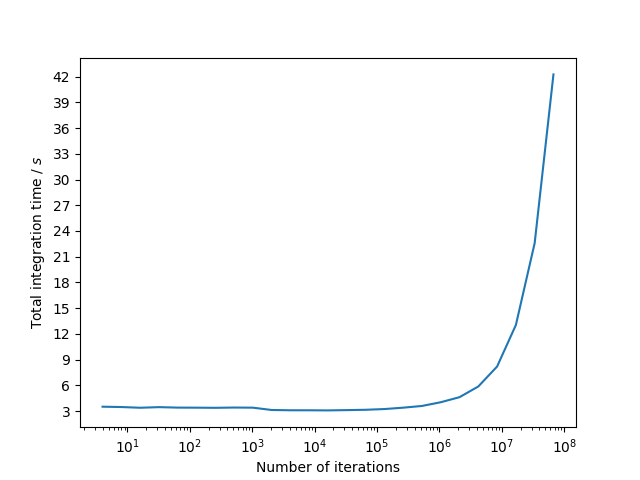
\includegraphics[width=\columnwidth]{NPlot.jpg}
	\caption{Time taken to integrate a simple DHO system for N timestep. The system has the parameters $r=4, \Delta t=0.01$s and has a lagrangian with the same form as equation \ref{DHOFamily} with $c_1=c_2=c_3=1$. Note that the number of iterations, N, is reported against a logarithmic scale and therefore the exponential growth seen for $N>10^6$ is a linear relationship between N and total integration time for $N$ in this region.}
\end{figure}

\subsection{Changing the order of the Integrator}
The order of the Slimplectic integrator,\cite{Tsang_Slimplectic}, is $r+2$ and allows us to approximate the error in the integrators predictions as
\begin{equation}
	|\textrm{Err}(\Delta t)| \approx a(\Delta t)^{r+2}.
\end{equation}

We can therefore increase the accuracy of the integrator by increasing $r$. Figure \ref{rplot} shows the effect of varying this for a Poynting-Robinson Drag system.

\todo{Finish this section off, talk to Josh and Gen data}

\begin{figure}
	\label{rplot}
	\includegraphics[width=\columnwidth]{pingu.jpg}
	\caption{ee}
\end{figure}

\subsection{Bounding the Integrator Error}
As with the original slimplectic integrator we investigate the fractional energy error relative to the analytic solutions energy. Here we observe almost identical behaviour to the original integrator. Mirroring figure 2 in Tsang et al. \cite{Tsang_Slimplectic} we compare the fractional energy error with the system evolution time for the JAX-based integrator and Runge-Kutta 2 and 4 methods. This is shown in figure \cite{EnergyPlot} and almost directly mirrors the original slimplectic integrators version of this figure. 

\begin{figure}
	\label{EnergyPlot}
	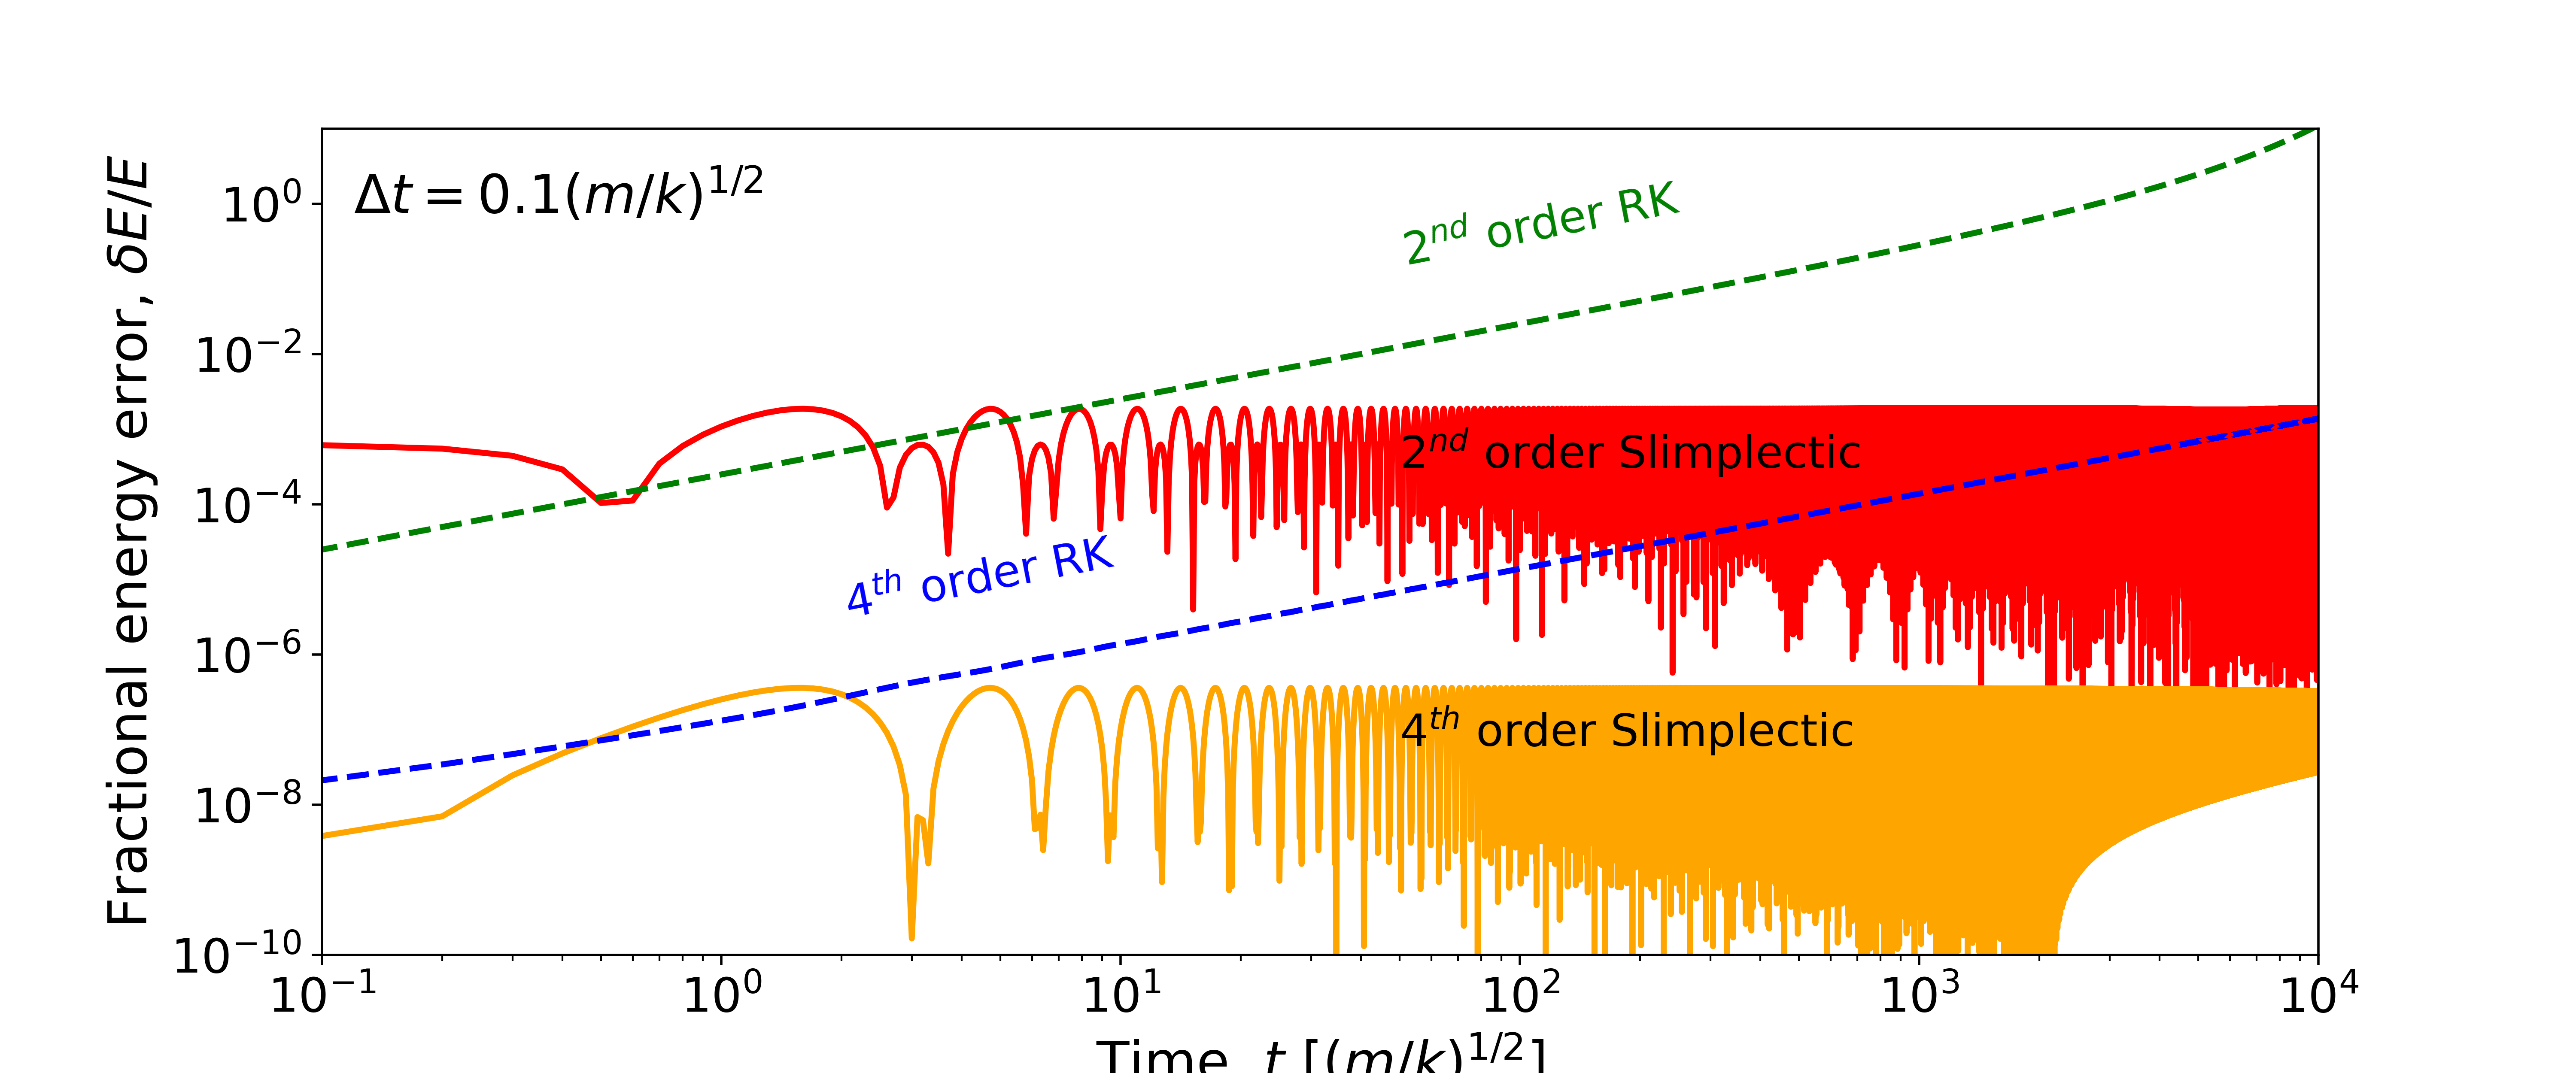
\includegraphics[width=\columnwidth]{EnergyPlot.png}
	\caption{ee}
\end{figure}

\subsection{Approximating DHO Functions}
We now move to the NN which was trained on a dataset of $5.0\times10^5$ randomly generated non-conservative lagrangians within the DHO family given by equation \ref{DHOFamily}. For each generated set of lagrangian coefficients, $\{c_1,c_2,c_3\}$, the conditions $c_1 > 0$ and $c_2,c_3 \geq 0$ were applied. Approximately $5\%$ of $c_2$ and $c_3$ values were randomly set to 0 such that the training dataset was guaranteed to have systems with $V,K = 0$. Negative values were discouraged through the implementation of an additional term in the loss function penalising coefficient values $ < -0.1$. This limit was chosen as to not discourage the neural network from choosing zero valued coefficients whilst still discouraging non-physical systems. 

Training of the model was temperamental and often susceptible to random permutations of the dataset causing diverging loss values which eventually broke models. By increasing batch sizes and introducing loss caps this was eventually remedied to produce a model that identifies trends within the data
\subsection{Differing Models}



\section{Discussion}
\section{Conclusion}
\ack
I would like to thank my project partner Joshua Coles for his indispensable coding abilities, ideas and overall support throughout this project. Without him I would still probably be stuck trying to set up the correct python environment. I would also like to thank my project supervisor Dr David Tsang. His advice and mentorship have been invaluable and I have very much enjoyed our often wandering discussions during project meetings. 
\section*{References}
\bibliographystyle{iopart-num}
\bibliography{references}

\end{document}
